\documentclass[22pt]{beamer}
\usepackage[orientation=portrait, size=custom, width=100.44, height=65,scale=1.2]{beamerposter} % 36in*2.5 = 90cm
\usepackage[absolute,overlay]{textpos}
\usepackage{bookmark} %pdflatex says to use this to avoid errors...
\usepackage{graphicx} %for including images
\graphicspath{{figs/}} %location of images
\usepackage{wrapfig} %wrap text around the images
\usepackage{listingsutf8}    %package for code environment; use this instead of verbatim to get automatic line break; use this instead of listings to get (•)
\usepackage{amsmath}
\usepackage{gensymb}
\usepackage[export]{adjustbox}
\usepackage[skins,theorems]{tcolorbox}
\usepackage{pgfplots}
\usepackage{tikz}
\usetikzlibrary{datavisualization}
\usetikzlibrary{datavisualization.formats.functions}
\usetikzlibrary{backgrounds}
\newcommand*\circled[1]{\tikz[baseline=(char.base)]{
            \node[shape=circle,draw,inner sep=2pt] (char) {#1};}}
\usepackage{array}
\usepackage{booktabs,adjustbox}
\usepackage{caption}
\captionsetup[figure]{font=scriptsize, labelfont=scriptsize}
\usepackage{ragged2e}
\usepackage{subfig}
\usepackage{xcolor}

%\mode<presentation>
%this doesn't seem to make any difference; leave for now for trying out
\usetheme{Berlin}
\definecolor{MacBlue}{rgb}{0.10196,0.22353,0.53725}
\definecolor{MacMaroon} {rgb}{0.47843, 0, 0.23137}
\definecolor{MacMaroon2} {rgb}{0.47451, 0, 0}
\definecolor{MacGray}{rgb}{0.50196,0.49804,0.51765}
\definecolor{MacMaroon3}{rgb}{00.47,0.2,0.31}
\definecolor{MacGold}{rgb}{1, 0.75,0.35}
\usecolortheme[named=MacBlue]{structure}
\setbeamertemplate{caption}[numbered]
\setbeamertemplate{navigation symbols}{}
% \setbeamercolor{background canvas}{bg=MacGray}

\title{Hakaru Language: Standard Library Implementation and Language Validation Testing}
\subtitle{}  %probably want a better subtitle
  \author[Justin Staples, Mahmoud Khattab, Nevin Mahilal and Aryan Sohrabi]{Justin Staples, Mahmoud Khattab, Nevin Mahilal and Aryan Sohrabi, supervised by Dr.~Christopher Anand \& Dr.~Jacques Carette \vspace{0.3cm} \newline \small \{staplejw, khattm, mahilank, sohraa3, anandc, carette\}@mcmaster.ca}
  \institute[McMaster University]{\small{Department of Computing and Software, McMaster University}}
  \date{}

\newenvironment{variableblock}[3]{%
  \setbeamercolor{block body}{#2}
  \setbeamercolor{block title}{#3}
  \begin{block}{#1}}{\end{block}}

\begin{document}
%compile with pdflatex

%there is only one frame, because there is only one page; yeah, it's a poster
%textblock and block seem to work nicely to organize layout
\begin{frame}[fragile]

\begin{textblock}{2}(0.8,0.9)

\includegraphics[height=8.5cm]{mac.png}
\end{textblock}

\begin{textblock}{2}(12.9,0.6)
\includegraphics[height=11cm]{fireball.png} 
\end{textblock}

\begin{textblock}{8}(4,1)
\titlepage
\end{textblock}

\begin{textblock}{5}(0.25,3.5)

%%%%%%%%%%%%%%%%%%%%%%%%%%%%%%%%%%%%%%%%%%%%%%%%%%%%%%%%%%%%%%%%%%%%%%
% Introduction
%%%%%%%%%%%%%%%%%%%%%%%%%%%%%%%%%%%%%%%%%%%%%%%%%%%%%%%%%%%%%%%%%%%%%%

\begin{block}{\Large{Introduction}}
\justifying

\bigskip
\normalsize{\textbf{Mathematical Background}}

\bigskip
\scriptsize{Consider a continuous random variable, \textit{X}, that is distributed according to a normal distribution. This is denoted by: }

\begin{equation*}
\begin{aligned}
& \tcboxmath[boxrule=2pt,colframe=MacMaroon]{\textit{X} \sim Normal(\mu, \sigma^2)}
\end{aligned}
\end{equation*}

\bigskip
\scriptsize{Below is a graph of the probability density function (PDF) for the standard normal distribution. It describes the probability that a sample of the random variable X will be equal to $x \in \mathbb{R}$.}

\bigskip
\scriptsize{The treatment of discrete random variables is much the same, except we refer to their probability mass function (PMF)}

\begin{figure}
\begin{tikzpicture}[framed, style={rounded corners}][>=stealth]
    \begin{axis}[
        xmin=-5,xmax=5,
        xtick={-5,-4,-3,-2,-1,0,1,2,3,4,5},
        xlabel=x,
        ymin=0,ymax=0.5,
        axis x line=middle,
        axis y line=middle,
        axis line style=<->,
    	width=0.8*\textwidth,
        height=1.2*\axisdefaultheight
        ]
        \addplot[no marks,blue,-] expression[domain=-5:5,samples=100]{1/sqrt(2*pi)*exp(-x^2/2)} 
                    node[pos=0.65,anchor=south west]{\textit{Normal(0, 1)}}; 
    \end{axis}
\end{tikzpicture}
\caption{\tiny{PDF of the normal distribution $^{[1]}$, with $\mu = 0$ and $\sigma = 1$}}
\end{figure}

\normalsize{\textbf{Language Guide}}

\bigskip
\scriptsize{Hakaru is an experimental \textbf{probabilistic programming language}, which aims to simplify the implementation of statistical distributions. 

\begin{itemize}
    \item Niche application means that Hakaru is a small language with limited features.
    \item Running a hakaru program generates a stream of random numbers distributed according the statistical distribution modeled.
    \item Hakaru code can be compiled to C and Haskell so that models can be exported for use in larger applications.
\end{itemize}

}

\bigskip
\scriptsize{{\tt \scriptsize{hk-maple}} is a provided inference algorithm that uses Maple to perform algebraic transformations on hakaru programs. In its default mode (Simplify), it returns an equivalent hakaru program with greater sampling efficiency. In applications requiring billions of samples (e.g. machine learning) this has the potential to save significant processing time!}

\end{block}

%%%%%%%%%%%%%%%%%%%%%%%%%%%%%%%%%%%%%%%%%%%%%%%%%%%%%%%%%%%%%%%%%%%%%%
% Key Concepts
%%%%%%%%%%%%%%%%%%%%%%%%%%%%%%%%%%%%%%%%%%%%%%%%%%%%%%%%%%%%%%%%%%%%%%

\begin{block}{\Large{Key Concepts}}
\justifying

\scriptsize{
\begin{itemize}
  \item[\textbf{$\star$}] \textit{Hakaru program $\Longleftrightarrow$ implementation of statistical distribution $\Longleftrightarrow$ probabalistic model $\Longleftrightarrow$ model.}
  \item[\textbf{$\star$}] \textit{Values pulled from a distribution are called measures. Measures $\Longleftrightarrow$ samples.}
  \item[\textbf{$\star$}] `{\textbf{$\sim$}}' vs `{\textbf{$<\sim$}}':
      \begin{itemize}
          \tiny
          \item[--] \tiny{$X \sim Normal(0, 1)$ means that the random variable, $X$, is distributed according to the standard normal distribution (statistics literature).}
          \item[--] \tiny{{\tt \tiny{x $<\sim$ normal(0, 1)}} means to pull a random variable from the standard normal distribution and bind it to the variable, {\tt \tiny{x}} (Hakaru code).}
      \end{itemize}
  \item[\textbf{$\star$}] \textit{PDF: Probability Density Function (continuous random variables).}
  \item[\textbf{$\star$}] \textit{PMF: Probability Mass Function (discrete random variables).}
  \item[\textbf{$\star$}] \textit{UDR chart: Univariate Distribution Relationship chart (describes relationships and transformations between different distributions).}
\end{itemize}
}
\end{block}

%%%%%%%%%%%%%%%%%%%%%%%%%%%%%%%%%%%%%%%%%%%%%%%%%%%%%%%%%%%%%%%%%%%%%%
% Motivation
%%%%%%%%%%%%%%%%%%%%%%%%%%%%%%%%%%%%%%%%%%%%%%%%%%%%%%%%%%%%%%%%%%%%%%

\begin{block}{\Large{Motivation}}
\justifying


\normalsize{\textbf{Objectives}}

\scriptsize{
\begin{itemize}
  \item Increase language accessibility: add new language features such as primivite mathematical functions (e.g. log, choose), new distributions, error handling, etc.
  \item Test language validity: use relationships between distributions to test the validity of program transformations like {\tt \scriptsize{hk-maple}}. 
\end{itemize}
}



\bigskip


\end{block}


\begin{textblock}{5}(5.5,3.5)

\begin{variableblock}{}{}{}
\justifying

\normalsize{\textbf{Endeavours}}

\scriptsize{
\begin{itemize}
  \item Standard library development: the UDR is used to branch out and implement new distributions. 
  \item Syntax-highlighting-for-hakaru package for Sublime Text: this package makes developing Hakaru code much more convenient and streamlined (Mahmoud).
  \item Test case writing: we focus mainly on comprehensively testing only a select few distributions (e.g. chi-square).
\end{itemize}
        }


\end{variableblock}


%%%%%%%%%%%%%%%%%%%%%%%%%%%%%%%%%%%%%%%%%%%%%%%%%%%%%%%%%%%%%%%%%%%%%%
% Standard Library Development
%%%%%%%%%%%%%%%%%%%%%%%%%%%%%%%%%%%%%%%%%%%%%%%%%%%%%%%%%%%%%%%%%%%%%%

\begin{block}{\Large{Standard Library Development}}
\justifying

\scriptsize{Accessibility means the standard library should implement commonly used probabilistic models. We have implemented the distributions described in the UDR chart, seen in part below. The following principles have guided the development of the standard library: 


\scriptsize{

\bigskip
\begin{itemize}
  \item Whenever possible, implement distributions as transformations on pre-existing models.
  \item Reference the UDR chart for possible ways to implement each distribution.
  \item In the case of multiple possible implementations, take the shortest possible path from a primitive distribution on the UDR.
\end{itemize}
        }
}

\bigskip

\begin{figure}
\centering
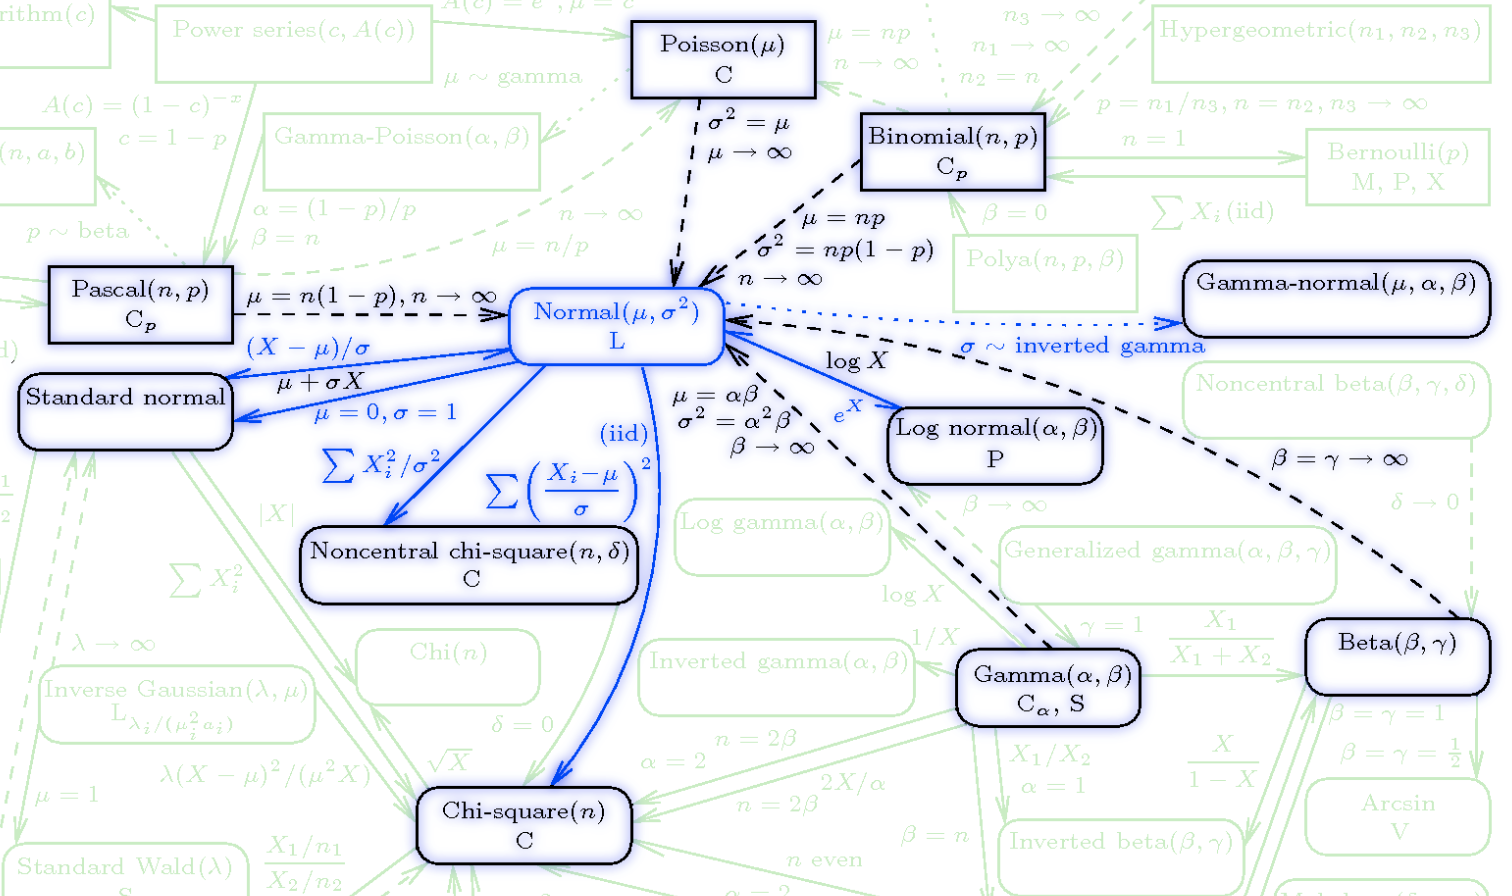
\includegraphics[height=12.5cm]{UDR.png}
\caption{\tiny{A snapshot of the UDR $^{[1]}$ shows how the normal distribution can be transformed into a multitude of other distributions.}}
\end{figure}

\scriptsize{Hakaru does not allow us to do algebraic operations on the PDF of a given distribution. The only operator we can use on a model is bind ({\tt \tiny{<$\sim$}}), to pull a sample and bind it to a variable (AKA a random variable). We are able to transform samples however we like. Therefore, we are interested in implementing transformations of the form:}

\begin{equation*}
\begin{aligned}
& \tcboxmath[boxrule=2pt,colframe=MacMaroon]{R(p, q) \Rightarrow \textit{X} \sim A(p) \Rightarrow \textit{f(X)} \sim B(q)}
\end{aligned}
\end{equation*}

\bigskip

\scriptsize{\textit{p} and \textit{q} are sets of parameters on the distributions \textit{A}} and \textit{B}. \textit{R(p, q)} is a set of relationships between \textit{p} and \textit{q} that must be satisfied. \textit{f} is a transformation on the random variable \textit{X}. We can extend this definition to include transformations defined in terms of an aggregation of multiple independent samples. For example, the standard chi-square distribution is defined as the sum of the squares of \textit{n} normal random variables (see Figure 3). 

\bigskip
\scriptsize{Hakaru also lends itself well to Bayesian transformations where we want to pull a sample from a distribution which is parameterized with a value sampled from another distribution. These transformations take the following form. Here, we are saying that if \textit{X} is parameterized by \textit{p}, then the distribution \textit{C}, which is parameterized by \textit{p} and \textit{q}, is equal to another distribution, \textit{B}, which is parameterized by \textit{q} and \textit{X}. The gamma-poisson distribution can be described by such a transformation (see Figure 4).}

\begin{equation*}
\begin{aligned}
& \tcboxmath[boxrule=2pt,colframe=MacMaroon]{X \sim A(p) \Rightarrow Y \sim B(q, X) = C(p, q)}
\end{aligned}
\end{equation*}

~
~
~

\bigskip
\begin{figure}
\centering
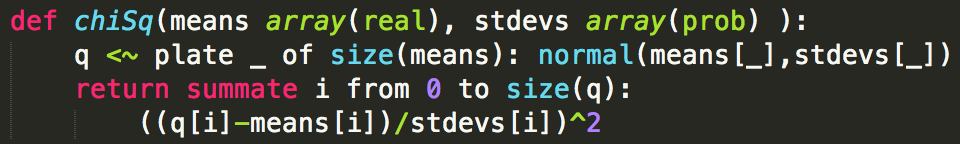
\includegraphics[height=3cm]{chi-square.png}
\caption{\tiny{Our implementation of the chi-square distribution.}}
\end{figure}

\end{block}



\end{textblock}

\end{textblock}


\begin{textblock}{5}(10.75,3.5)

\begin{variableblock}{}{}{}
\justifying

\bigskip
\begin{figure}
\centering
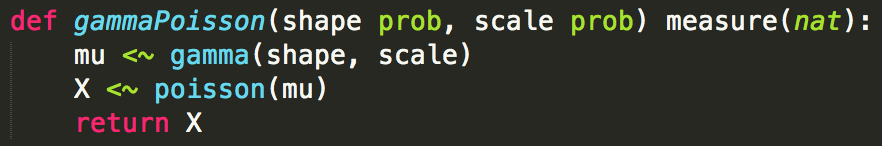
\includegraphics[height=3cm]{gamma-poisson.png}
\caption{\tiny{Our implementation of the gamma-poisson distribution.}}
\end{figure}

\scriptsize{Some distributions on the UDR are unreachable from Hakaru's primitive distributions using transformations like the 2 described above. In these cases, we have to implement the model in terms of the PMF for a discrete distribution or in terms of the PDF for a continuous distribution.}

\bigskip
\scriptsize{

A Python script has been developed that samples a large amount of data and plots the results in a histogram. This is a useful tool for gaining confidence in the correctness of our implementations. The plots shown below were created by sampling a Hakaru program 1,000,000 times. 
}

\begin{figure}[!tbp]
  \centering
  \subfloat[]{ 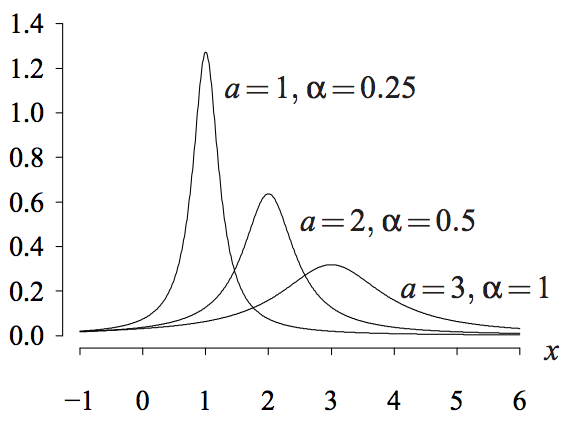
\includegraphics[width=0.38\textwidth]{cauchy.png}\label{fig:f1}}
  \subfloat[]{ 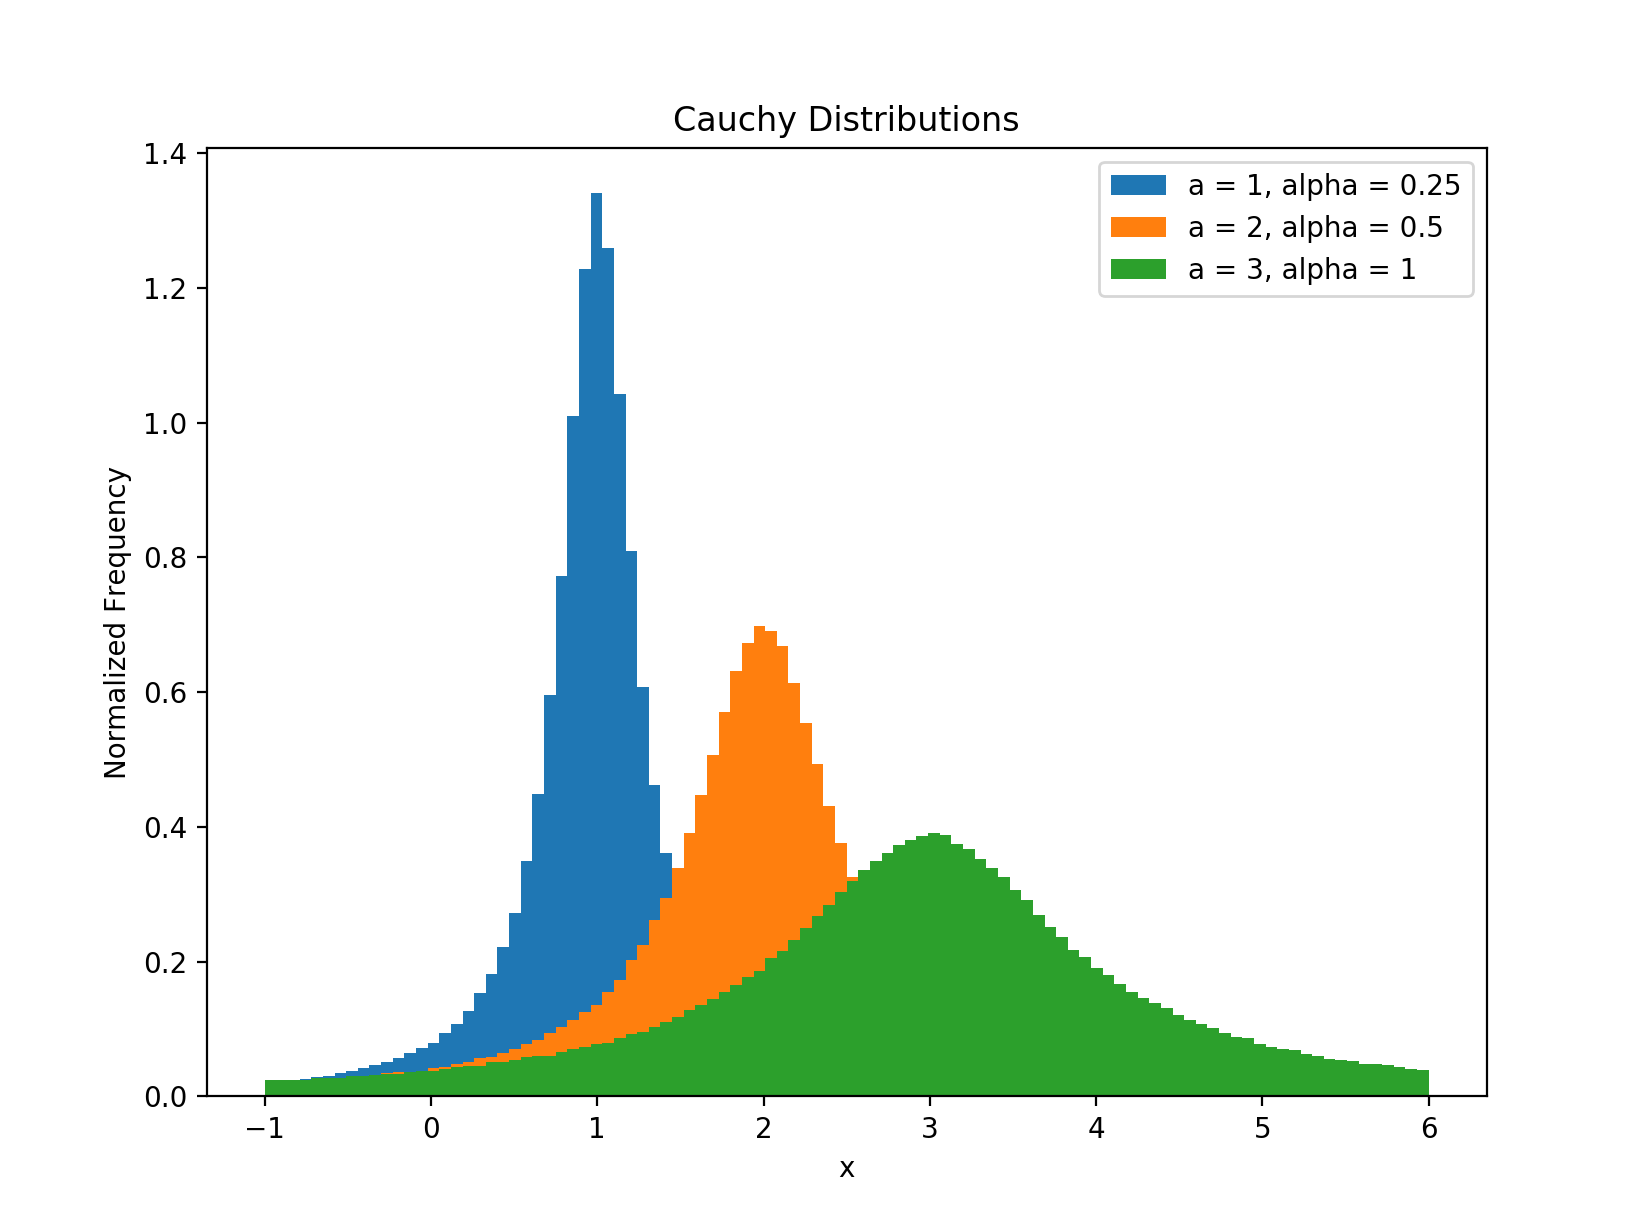
\includegraphics[width=0.38\textwidth]{cauchy_2.png}\label{fig:f2}}
  \caption{\tiny{A few plots of the Cauchy distribution are shown $^{[1]}$, along with a few histograms of data that have been sampled from a Hakaru program.}}
\end{figure}


\end{variableblock}

%%%%%%%%%%%%%%%%%%%%%%%%%%%%%%%%%%%%%%%%%%%%%%%%%%%%%%%%%%%%%%%%%%%%%%
% Testing Relationships Between Distributions
%%%%%%%%%%%%%%%%%%%%%%%%%%%%%%%%%%%%%%%%%%%%%%%%%%%%%%%%%%%%%%%%%%%%%%

\begin{block}{\Large{Testing Relationships Between Distributions}}
\justifying

\scriptsize{When developing the standard library, the UDR chart often implied multiple possible implementations for a given distribution. We expect alternative implementations for the same distribution to result in equivalent probabilistic models. This line of thought is the basis for the kinds of test cases implemented. More generally, we have the following hypothesis.}

\bigskip

\scriptsize{Assume we know a proven relationship between 2 statistical distributions, A and B, which allows us to transform A and B into distributions that are equivalent to each other. Further assume this transformation takes on one of the forms discussed in the Standard Library Development section. We hypothesize that by applying the appropriate transformations to implementations of A and B, we can create two Hakaru programs whose {\tt \scriptsize{hk-maple}} outputs will be equivalent to each other. Test cases that prove our hypothesis true indicate the validity of the Hakaru language implementation. Test cases that prove our hypothesis false indicate an underlying bug in the language definition which is to be passed back to the language developers.
}

\end{block}

%%%%%%%%%%%%%%%%%%%%%%%%%%%%%%%%%%%%%%%%%%%%%%%%%%%%%%%%%%%%%%%%%%%%%%
% Conclusions & Future Work
%%%%%%%%%%%%%%%%%%%%%%%%%%%%%%%%%%%%%%%%%%%%%%%%%%%%%%%%%%%%%%%%%%%%%%

\begin{block}{\Large{Conclusions \& Future Work}}

\scriptsize{This project was aimed at increasing language accessibility and testing the validity of Hakaru. A lot of ground was covered in both of these aspects in this project, but compared to other popular languages, Hakaru is still under development and has a lot of room for improvement. Here are just a few examples of where major development can still be done.

\begin{itemize}
    \item Languages features: Hakaru can be expanded further with new features like import statements and error/exception handling. 
    \item Standard library development: there are still many types of  distributions left to be implemented, such as multivariate distributions.
    \item Testing: There are a plethora of relationships between distributions that have yet to be investigated.  
\end{itemize}

}

\end{block}

%%%%%%%%%%%%%%%%%%%%%%%%%%%%%%%%%%%%%%%%%%%%%%%%%%%%%%%%%%%%%%%%%%%%%%
% References
%%%%%%%%%%%%%%%%%%%%%%%%%%%%%%%%%%%%%%%%%%%%%%%%%%%%%%%%%%%%%%%%%%%%%%

\begin{block}{\Large{References}}

\scriptsize{[1]~L. Leemis, "Univariate Distribution Relationship Chart", Math.wm.edu, 2018. [Online]. Available: http://www.math.wm.edu/~leemis/chart/UDR/UDR.html. 

[2]~P. Narayanan, J. Carette, W. Romano, C. Shan and R. Zinkov, “Probabilistic Inference by Program Transformation in Hakaru (System Description)”, Functional and Logic Programming, pp. 62-79, 2016.}


\end{block}


% \begin{block}{References}
% \setbeamertemplate{bibliography item}{\insertbiblabel}
% \bibliographystyle{ieeetr}
% {\scriptsize
% \bibliography{../bib}}
% \end{block}

\end{textblock}
\end{frame}
\end{document}
